\documentclass[xcolor=dvipsnames, 14pt]{beamer}
\usetheme{Darmstadt}
\usecolortheme[named=Peach]{structure}

% balíčky

\usepackage[utf8]{inputenc}
\usepackage[czech]{babel}
\usepackage{graphicx}

% informace o dokumentu

\title[Synchronizace a replikace geodat]{Synchronizace a replikace geodat \\v prostředí Esri platformy}
\author[RNDr. V. Pechanec, Ph.D., M. Solanská]{RNDr. Vilém Pechanec, Ph.D. \\Markéta Solanská}
\date[6.3.2013]{1. diplomový den, 6.3.2013}


% text dokumentu

\begin{document}

% titulní stránka
% (název prezentace, autor, datum...)

\begin{frame}
  \titlepage
\end{frame}

% osnova prezentace
% (většinou se pro délku vypouští)

% obsah prezentace
% (používají se klasické sekce)

\section{Synchronizace a replikace geodat v prostředí Esri platformy}

  \begin{frame}
    \frametitle{Cíle práce}
    \framesubtitle{Teoretická část}
    \begin{itemize}
      \item definování procesů synchronizace a replikace
      \item popis prostředků pro synchronizaci a replikaci využívaných Esri produkty
      \item popis požadavků, možností a předpokladů pro správný průběh těchto procesů
      \item popsat řešení pro ArcGIS for Desktop, ArcGIS for Server, ArcGIS online
    \end{itemize}
  \end{frame}

  \begin{frame}
    \frametitle{Cíle práce}
    \framesubtitle{Praktická část}
    \begin{itemize}
      \item praktické otestování procesů replikace a synchronizace na Esri produktech
      \item testování: rychlosti procesu, úplnosti, chybovosti, kvality, podporovaných formátů
      \item databáze: SQL Server Express 2008\\ \hspace{19.5mm} PostgreSQL 9.x
      \item data: environmentální data Litovelského Pomoraví
    \end{itemize}
  \end{frame}

  \begin{frame}
    \frametitle{Replikace}
    \begin{itemize}
      \item replikace zajišťuje kopii dat a synchronizaci změn z jednoho serveru na druhý
      \item využití:
        \begin{itemize}
        \begin{normalsize}
          \item záloha serveru při výpadku či ztrátě dat
          \item snížení zátěže serveru
          \item sdílení dat dvou a více databází
        \end{normalsize}
        \end{itemize}
      \item synchroní x asynchronní replikace
      \item jednosměrná x obousměrná replikace
    \end{itemize} 
  \end{frame}

  \begin{frame}
    \frametitle{Replikace}
    \begin{itemize}
      \item master-slave replikace
      \\  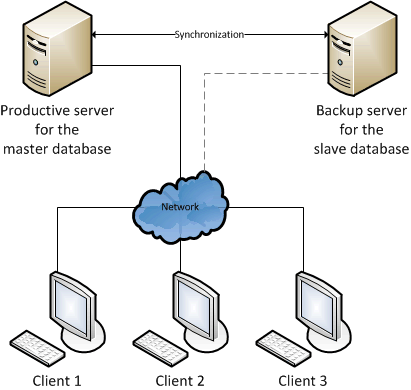
\includegraphics[scale=0.5]{obr/db_replikation.png} 
      \\  \begin{tiny}(zdroj:http://www.passwordsafe.de/uploads/pics/db\_replikation\_EN.gif)\end{tiny}
    \end{itemize} 
  \end{frame}

  \begin{frame}
    \frametitle{Technologie ArcSDE}
    \framesubtitle{ESRI produkty}
    \begin{itemize}
        \item prostředník pro komunikaci mezi klientem a SQL databází (př. ArcGIS for Desktop a PostgreSQL)
        \item technologie pro přístup a správu geografických dat v relační databázi
        \item umožňuje současnou editaci jedné databáze více uživateli
        \item podpora OGC a ISO standardů
    \end{itemize} 
  \end{frame}

  \begin{frame}
    \frametitle{Technologie ArcSDE}
    \framesubtitle{ESRI produkty}
    \begin{itemize}
        \item podpora databázových systémů:
          \begin{itemize}
          \begin{normalsize}
            \item DB2
            \item Informix
            \item Oracle
            \item PostgreSQL
            \item SQL Server and SQL Server Express
          \end{normalsize}
          \end{itemize}
    \end{itemize} 
  \end{frame}

  \begin{frame}
    \frametitle{Výstup diplomové práce}
    \begin{itemize}
      \item popis procesu replikace a synchronizace a souhrn jejich pořadavků u Esri produktů
      \item porovnání procesů s použitím SQL Server Express a PostgreSQL
      \item hodnocení procesů na základě testování rychlosti, kvality, spolehlivosti, úplnosti, ...
    \end{itemize}
  \end{frame}
  
  \begin{frame}
    \begin{center}
      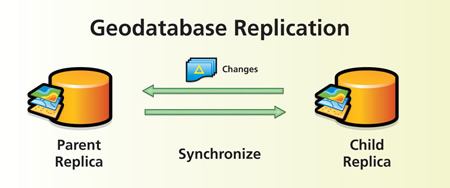
\includegraphics[scale=0.5]{obr/replication.jpg} 
      \\  \begin{tiny}(zdroj:http://www.esri.com)\end{tiny}
    \\ \huge{Děkuji za pozornost.}
    \end{center}
  \end{frame}

\end{document}
